

\documentclass[conference,12pt]{IEEEtran}
\usepackage{blindtext, graphicx}
\usepackage[]{graphicx}
\usepackage[sort, numbers]{natbib}
\usepackage{hyperref}
\usepackage{adjustbox,lipsum}
\usepackage{subfig}
\usepackage{float}
\usepackage{amssymb,amsmath}
\usepackage{textcomp}


\hyphenation{op-tical net-works semi-conduc-tor}


\begin{document}
%
% paper title
% can use linebreaks \\ within to get better formatting as desired
\title{GeoSched: Minimizing Cost of Cloud Workloads in Geo-Distributed Data Centers}


% author names and affiliations
% use a multiple column layout for up to three different
% affiliations
\author{\IEEEauthorblockN{Anirudh Jayakumar}
\IEEEauthorblockA{Department of Computer Science\\
University of Illinois at Urbana-Champaign\\
Email: ajayaku2@illinois.edu}
\and
\IEEEauthorblockN{Harshit Dokania}
\IEEEauthorblockA{Department of Computer Science\\
University of Illinois at Urbana-Champaign\\
Email: hdokani2@illinois.edu}
}

% conference papers do not typically use \thanks and this command
% is locked out in conference mode. If really needed, such as for
% the acknowledgment of grants, issue a \IEEEoverridecommandlockouts
% after \documentclass

% for over three affiliations, or if they all won't fit within the width
% of the page, use this alternative format:
% 
%\author{\IEEEauthorblockN{Michael Shell\IEEEauthorrefmark{1},
%Homer Simpson\IEEEauthorrefmark{2},
%James Kirk\IEEEauthorrefmark{3}, 
%Montgomery Scott\IEEEauthorrefmark{3} and
%Eldon Tyrell\IEEEauthorrefmark{4}}
%\IEEEauthorblockA{\IEEEauthorrefmark{1}School of Electrical and Computer Engineering\\
%Georgia Institute of Technology,
%Atlanta, Georgia 30332--0250\\ Email: see http://www.michaelshell.org/contact.html}
%\IEEEauthorblockA{\IEEEauthorrefmark{2}Twentieth Century Fox, Springfield, USA\\
%Email: homer@thesimpsons.com}
%\IEEEauthorblockA{\IEEEauthorrefmark{3}Starfleet Academy, San Francisco, California 96678-2391\\
%Telephone: (800) 555--1212, Fax: (888) 555--1212}
%\IEEEauthorblockA{\IEEEauthorrefmark{4}Tyrell Inc., 123 Replicant Street, Los Angeles, California 90210--4321}}




% use for special paper notices
%\IEEEspecialpapernotice{(Invited Paper)}

\newenvironment{list1}{
  \begin{list}{\ding{113}}{%
      \setlength{\itemsep}{0in}
      \setlength{\parsep}{0in} \setlength{\parskip}{0in}
      \setlength{\topsep}{0in} \setlength{\partopsep}{0in}
      \setlength{\leftmargin}{0.17in}}}{\end{list}}
\newenvironment{list2}{
  \begin{list}{$\bullet$}{%
      \setlength{\itemsep}{0in}
      \setlength{\parsep}{0in} \setlength{\parskip}{0in}
      \setlength{\topsep}{0in} \setlength{\partopsep}{0in}
      \setlength{\leftmargin}{0.2in}}}{\end{list}}

% make the title area
\maketitle


\begin{abstract}
%\boldmath
Today, many of the leading cloud service providers have geographically distributed data centers to serve millions of users around the world. The need for a geo-distributed data center arises from the need to provide low-latency and  high-availability of the different services. The workloads that run on these data centers are also highly diverse. A typical data centers run jobs of different kinds including business-critical workloads---web servers, mail servers, instant messaging services etc, big-data processing, real-time data analytics and HPC jobs. As cloud services grow to serve more customers, there is an increasing need for a workload provisioning mechanism which can minimize the cost of operation of the data center while minimizing SLA violations and also minimizing the user-perceived latency. 

We present GeoSched, a job provisioning framework that is workload aware, energy-aware and cooling-aware. GeoSched considers the latency sensitivity of the incoming jobs, electricity pricing of the region and cooling techniques used in the data center to schedule jobs on different data centers. To evaluate our scheme, we perform extensive simulations on real-world workload traces.
\end{abstract}
% IEEEtran.cls defaults to using nonbold math in the Abstract.
% This preserves the distinction between vectors and scalars. However,
% if the journal you are submitting to favors bold math in the abstract,
% then you can use LaTeX's standard command \boldmath at the very start
% of the abstract to achieve this. Many IEEE journals frown on math
% in the abstract anyway.

% Note that keywords are not normally used for peerreview papers.
\begin{IEEEkeywords}
Cloud Computing, Energy consumption, Resource management, Data center.
\end{IEEEkeywords}


\section{INTRODUCTION}
\label{sec:intro}
The emergence of cloud computing has resulted in an array of services being provided over the Internet. These services include office applications, raw compute power, storage and a variety of Internet services including social media, multimedia streaming among many others. Also due to the explosion of digital content, big data, e-commerce, and Internet traffic, there is a continuous effort to expand the capacity of data centers. This demand has increased the need for efficient data centers to handle the large amount computing resource requests especially among Internet companies like Facebook, Google, Microsoft and Amazon. The size of these data centers can be more than 100,000 servers \cite{greenberg2008cost} resulting in a huge costs, both to procure the IT infrastructure and to keep the systems running.

A typical data center consists of three major subsystems: servers and network cables form the IT equipments, power subsystem that supports the data center and the cooling equipments that help to maintain the temperature of the data center for the IT equipments to work effectively. The amount of energy required to smoothly run a data center is extremely high. In 2013 alone, U.S data centers have consumed 91 billion kilowatt-hours of electricity \cite{nrdcreport}, which is the amount of electricity needed to power New York City twice over. This energy consumption is expected to reach 140 billion kilowatt-hours by 2020. A major part of the energy consumption is due to cooling energy, the energy required to maintain a specific temperature in the data center. According to some reports the cooling energy can be as high as 50\% \cite{sullivan2002alternating} \cite{patel2003smart} \cite{sawyer2004calculating} of the total energy budget. 

In this paper we propose a meta-scheduler which schedules jobs to those data center which will cost the least to run an incoming job. This will in-turn reduce the total cost of operations and can benefit enterprises that operate geo-distributed data centers. Our scheduler take into account the server running costs as well as the cooling costs. The cooling costs depends on the kind of equipment used. In a traditional data center, chillers are used to cool down the hot air from CRAC units using mechanical refrigeration. This mechanism incurs large amount of power \cite{zhou2012optimization}. Recently, most data centers have adopted very cost effective mechanism called air-side economizer to cool the servers. An air-side economizer pulls the outside air into the data center and the hot air is directed outside, thus cooling the IT equipments in the data center. The use of such economizer is restricted to cooler regions. We exploit the fact that geo-distributed data centers will have different temperatures and hence the cooling efficiency of data centers will differ. 
%Last line

The rest of the paper is organized as follows. Section \ref{sec:related} presents the related work on cost minimization of data centers and other energy-efficiency research in the cloud computing. Section \ref{cloudworkload} provides a description of the workloads used in our experiments. Section \ref{sec:datacenter} gives details of the data center profiling which we did to emulate real-world data centers. Section \ref{sec:sysmodel} defines the system model. Section \ref{sec:conclusion} provides details of the experiments and Section \ref{sec:eval} concludes the paper with discussion and future work. 

   


%%%%%%%%%%%%%%%%%%%%%%%%%%%%%%%%%%%%%%%%%%%%%%%%%%%%%%%%%%%%%
\section{RELATED WORK}
\label{sec:related} 
Cost minimization has been extensively studied both in the context of a single data center and a geo-distributed data center. Most of the work has been targeted towards minimizing the energy consumption of the data center to reduce the operational cost. For example, the work by Gu \textit{et al.} \cite{gu2014cost} studies the influence of task assignment, data placement  and data movement on the operational expenditure of large-scale geo-distributed data centers for big data applications. The authors jointly optimize  these three factors by proposing a 2-D Markov chain to derive the average task completion time and solve the model as a MILP problem. On similar lines Agarwal \textit{et al.} \cite{agarwal2010volley} propose an automated data placement mechanism Volley for geo-distributed cloud services with the consideration of WAN bandwidth cost, data center capacity limits, data inter-dependencies, etc. 

Yu \textit{et al.}\cite{yu2015energy} propose minimizing energy cost for distributed Internet data centers (IDCs) in smart microgrids by considering system dynamics like uncertainties in electricity price, workload, renewable energy generation, and power outage state. They model the problem as a stochastic program and solve it using Lyapunov optimization technique. The work by Ren and He  \cite{ren2013coca} propose an online algorithm, called COCA to minimize data center operational cost while satisfying carbon neutrality. Unlike some of the existing research, COCA enables distributed server-level resource management: each server autonomously adjusts its processing speed and optimally decides the amount of workloads to process. This work is restricted to a single data center with heterogeneous resources. 

Cooling energy is a substantial part of the total energy spent by a data center. According to some reports, this can be as high as 50\% \cite{sullivan2002alternating}, \cite{patel2003smart},\cite{sawyer2004calculating} of the total energy budget. There has been a lot of work both at the application/middleware level \cite{TempLDBSC11}, \cite{leverich2010energy} as well as provisioning techniques  \cite{tang2007thermal}, \cite{chen2010integrated} that try to minimize the cooling energy.   

Other research related to cooling efficiency include the work by Liu \textit{et al.} \cite{liu2012renewable}  that reduces electricity cost and environmental impact using a holistic approach that integrates renewable supply, dynamic pricing, and cooling supply including chiller and outside air cooling, with IT workload planning to improve the overall sustainability of data center operations. The authors first predict renewable energy as well as IT demand. Then they use these predictions to generate an IT workload management plan that schedules IT workload and allocates IT resources within a data center according to time varying power supply and cooling efficiency. This is done in the context of a single data center.

\iffalse
Pakbaznia and Pedram \cite{pakbaznia2009minimizing} focuses on minimizing power for both IT equipment and air conditioning power usage. The authors consider both server consolidation and task assignment together and formulate the resulting optimization problem a a ILP problem and present a heuristic algorithm that loves it in polynomial time.

There are also research done to look at the impact of failures in data centers on the operational cost. The work by Cui \textit{et al.} \cite{cui2014shadows} considers the increase in energy consumption due to failures in large scale clouds. A slower shadow replication of the main process is used to recover from faults thereby saving energy up to 30\%. Guenter \textit{et al.} \cite{guenter2011managing} also considers different trade-offs between cost, performance and reliability to formulate an optimization problem that minimizes energy costs, reliability costs and unmet demands. VM migration techniques are also used extensively to increase the energy efficiency of cloud data centers. One such approach is proposed by Rodero \textit{et al.} \cite{rodero2012energy} where the author  propose to use application profiling (CPU, memory, bandwidth) to  design application-centric energy-aware strategy for VM allocation during VM migration.

Researchers have also studied the efficient use of green energy in data centers. Goiri \textit{et al.} \cite{goiri2011greenslot} propose a system GreenSlot that maximizes the use of green energy available at data centers while ensuring all job deadlines are met. GreenSlot predicts the solar energy available in data centers in near future and schedules the workload to maximize green energy consumption and meeting jobs deadlines. Green- Slot can increase green energy consumption by up to 117\% and decrease energy cost by up to 39\%, compared to a conventional scheduler. 

\fi

%%%%%%%%%%%%%%%%%%%%%%%%%%%%%%%%%%%%%%%%%%%%%%%%%%%%%%%%%%%%%


%%%%%%%%%%%%%%%%%%%%%%%%%%%%%%%%%%%%%%%%%%%%%%%%%%%%%%%%%%%%%


\section{CLOUD WORKLOADS } \label{cloudworkload}
With the increase in the adoption of cloud computing by businesses around the world, more and more workloads are moving out of traditional data centers into the cloud. A cloud data center typically handles a range of IT workloads. These workloads include service-critical and latency sensitive interactive applications that run 24x7 such as instant messengers, e-mail applications and other Internet services, and batch-style applications such as scientific HPC applications, Big Data applications like financial analysis and Map Reduce applications. A thoughtful management of these workloads are necessary not only to provide customers with low-latency services but also to reduce the energy consumption of the data centers that run these workloads. A good way to study these workloads are by analyzing real-world or synthetic workload traces. We look at cloud workload traces in detail in section \ref{traces} and \ref{googletrace}

\subsection{Workload Traces} \label{traces}
Unfortunately, there is a lack of real-world traces in the cloud computing research community. As a result, there are limited work done to understand the diversity in cloud workloads. The first large-scale workload trace was released by Google in 2011\cite{googletracedata}, featuring traces from over 12,000 servers over a period of 29 days. Various studies have been carried out to understand the characteristic of the Google trace data. Other real-world traces include Wikipedia request trace \cite{urdaneta2009wikipedia} and Hadoop logs from Yahoo! \cite{yahootrace}There have also been attempts to generate synthetic workload traces using known real-world workload characteristics \cite{beitch2010rain} \cite{wang2011towards}. For our experiments we use the workload trace from Google. 

\subsection{Custom Trace Format}
To have a common trace format to represent different real-world and synthetic workload traces, we have formulated a trace format similar to standard workload format (swf) \cite{chapin1999benchmarks} defined for grid and supercomputing traces. Table \ref{tab:format} provides information about each field in the trace format. The format provides a uniform schema that can be used by different cloud providers to supply their workload traces. This can also be used as a common input format by various scheduling simulators. Our simulator, \textit{GeoSim} which is explained in section \ref{sec:simdesign} also used this format to represent jobs.
 
\begin {table}[]
\centering
 \scalebox{0.85}{\begin{tabular}{ | p{2.5cm} |l  |p{6 cm}|  }
    \hline
    \bf{Field Name} & \bf{Type} & \bf{Description}   \\ \hline
     JobID & INT  & Unique job identifier for each job\\ \hline
     Arrival Time & INT & Arrival time in microseconds \\ \hline
     Scheduled Time & INT  & Arrival time in microseconds\\ \hline
     Finish Time & INT  & Arrival time in microseconds\\ \hline
     Schedule class & INT  & Latency class of the job. \\ \hline
     Tasks & INT  & Total number of tasks in the job. \\ \hline
     Total CPU& INT  & Aggregate sum of CPU used by all the tasks in the job\\ \hline
     Total Memory& INT   & Aggregate sum of memory used by all the tasks in the job \\ \hline
     User& INT  & Unique user identifier \\ \hline
     SLA Param1&  FLOAT & SLA parameter placeholder\\ \hline
     SLA Param2&  FLOAT & SLA parameter placeholder\\ \hline
     SLA Param3&  FLOAT & SLA parameter placeholder\\ \hline
    \end{tabular}}
    \caption {Trace format description} \label{tab:format} 
\end{table}

\subsection{Google Workload Trace} \label{googletrace}
Google trace has job and task information in different files. We consolidated all the required information and generated a single work trace file with the format described in the previous section. For our work, we model five different data centers located at different parts of the globe. A detailed explanation about the data center profile are given in section \ref{sec:datacenter}. To simulate workload execution in these five data centers we have extracted five set of traces each worth five days of incoming job requests from the original Google trace. This will cover 25 days of traces out of the 29 available days. We label these 5 set of traces from A to E.   Additionally,  in our  experiments  we  only  consider  those  jobs  that end  without  any  failures.  Therefore,  we  clean  the original  traces  by  removing  all  jobs  that  have  either failed or got killed. The left over 4 days of the workload is used to gain statistical user related insights to predict the running time of incoming jobs. 

\begin{figure}[] 
\centering
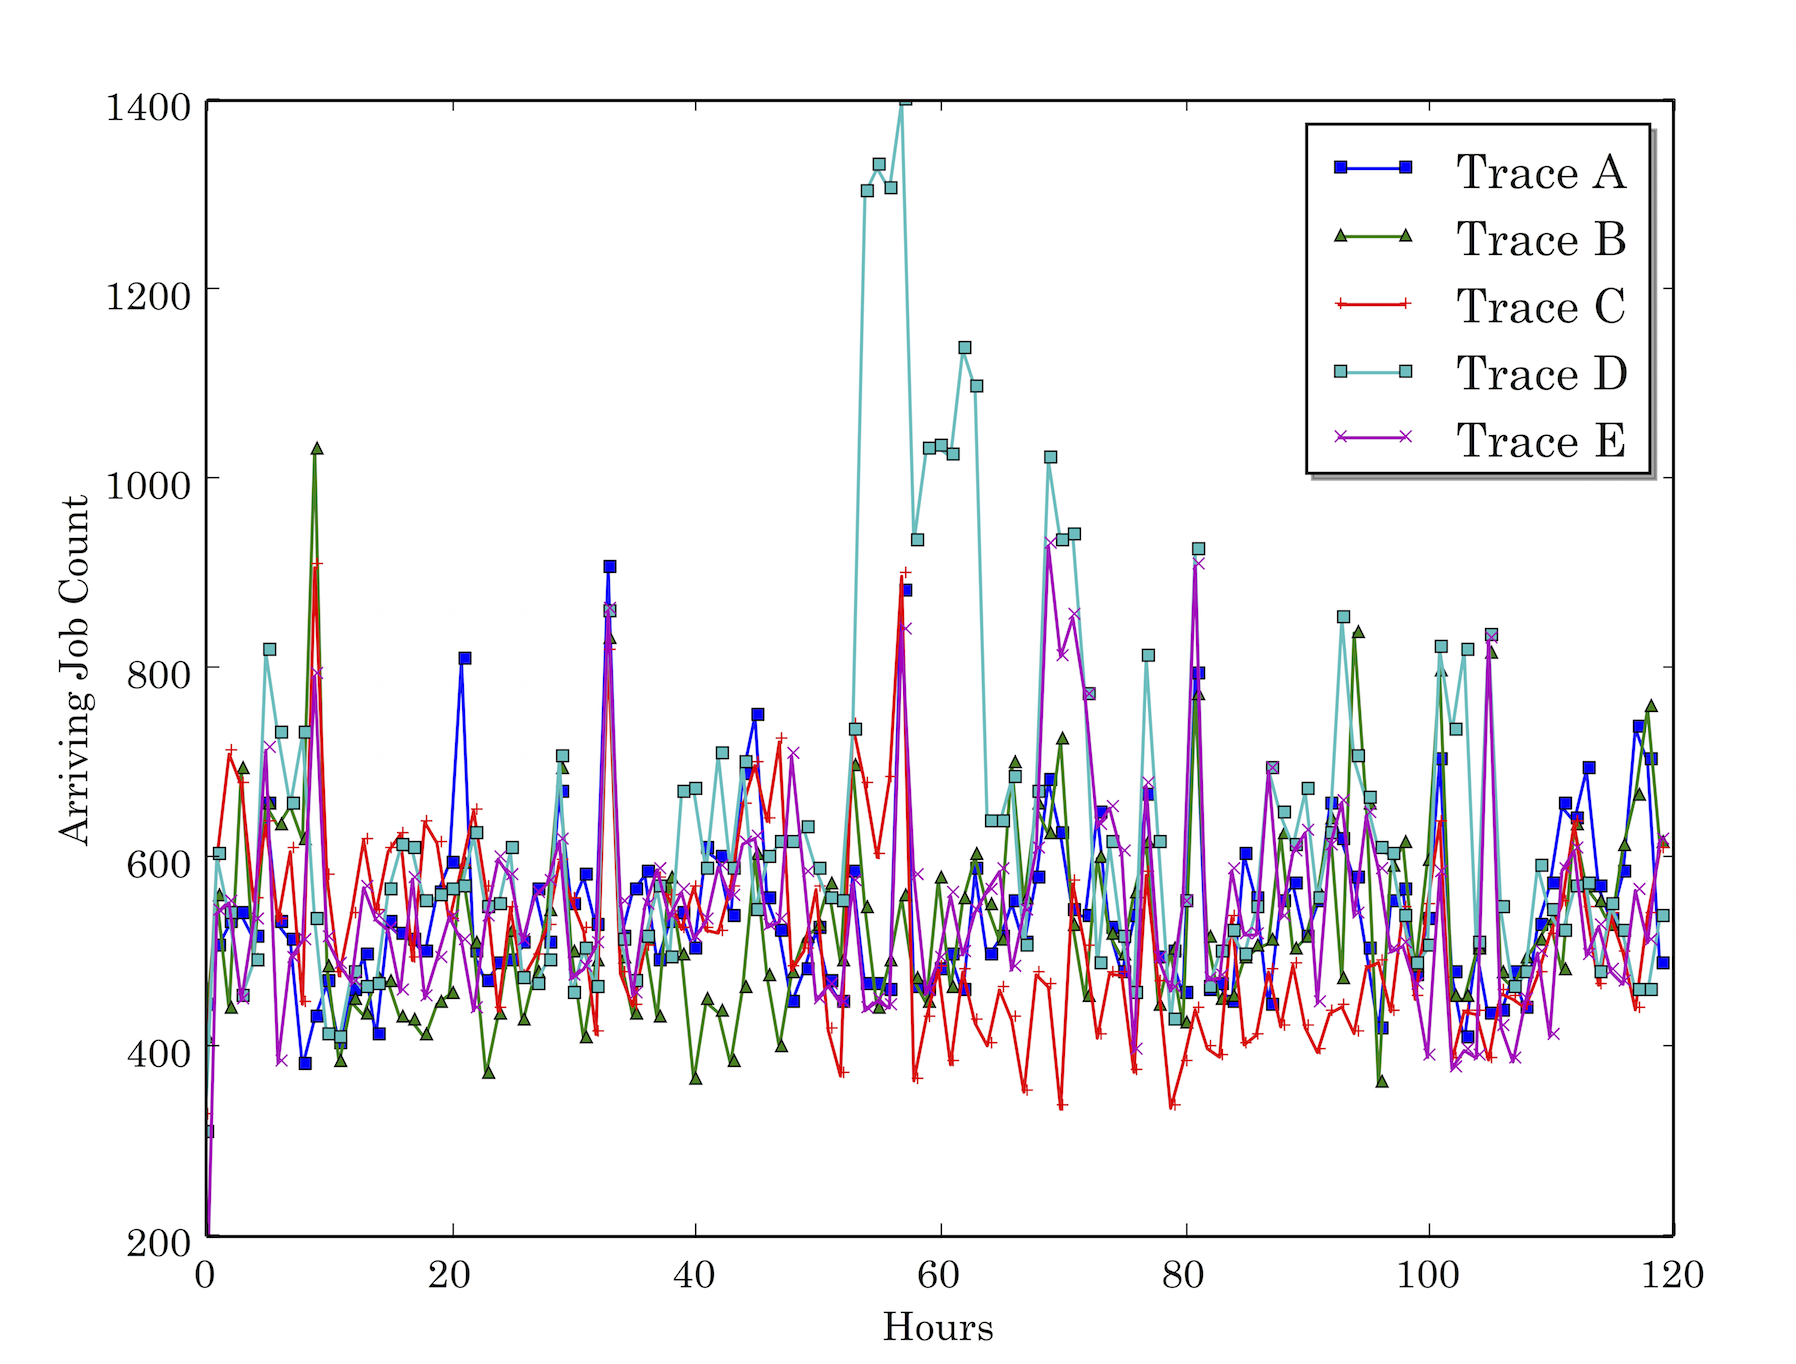
\includegraphics[scale=0.3]{arrivalrate.png}
\caption{Arrival rate of jobs }
\label{fig:arrivalrate}
\end{figure}

Now we will look at some characteristics of the traces. Table \ref{tab:tracestat} describes the statistics for each of the five traces grouped by the scheduling class of the job. In Google traces, CPU and memory usage are normalized relative to the largest capacity of the resource on any machine in the trace (which is 1.0). Most of the class 0 and class 1 jobs are batch jobs with less latency requirements. Generally, these are the kind of jobs that can be provisioned on other data centers as their deadlines are not strict.  You will find that as the sensitivity increases the running time of these jobs and the resource usage also increase. High-sensitive jobs are generally service jobs and run of longer periods of time. Figure \ref{fig:pie} shows a pie chart of the job counts in different schedule classes for all the 5 traces. You will notice that the job count for class 3 (high latency-sensitive) jobs are low. This is because these jobs generally run for long period of time, typically months. Since we only consider jobs that start and end within the 29 day range such jobs are missed out in our traces. For our work, we will consider class-0 and class-1 jobs as candidates for optimizing the provisioning. Class-2 and class-3 jobs are provisioned to run on the data center where the job arrived since these are high-sensitive and their SLA demands will be strict. 


\begin{figure*}[]
\centering
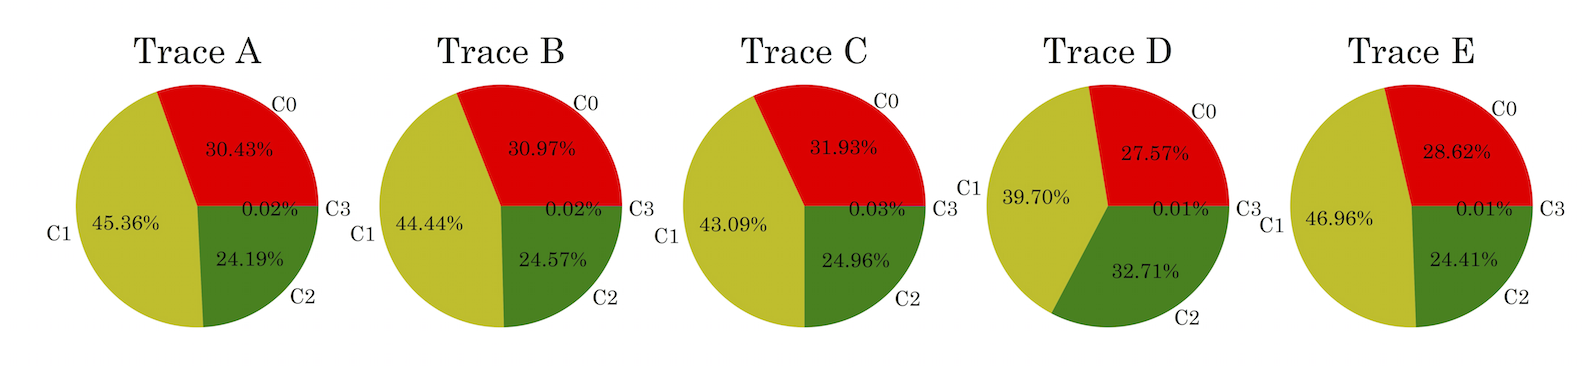
\includegraphics[scale=0.65]{pie}
\caption{ Distribution of job count in various schedule classes}
 \label{fig:pie}
\end{figure*}

\begin{table*}[]
\adjustbox{max width=1\textwidth}{

\begin{tabular}{|l|l|l|l|l|l|l|l|l|l|l|l|l|l|l|l|}
\hline
 & \multicolumn{3}{l|}{\bf{Trace A}} & \multicolumn{3}{l|}{\bf{Trace B}} & \multicolumn{3}{l|}{\bf{Trace C}} & \multicolumn{3}{l|}{\bf{Trace D}} & \multicolumn{3}{l|}{\bf{Trace E}} \\ \hline
\textbf{\begin{tabular}[c]{@{}l@{}}Sched\\ Class\end{tabular}} & \textbf{\begin{tabular}[c]{@{}l@{}}Avg \\ CPU\end{tabular}} & \textbf{\begin{tabular}[c]{@{}l@{}}Avg\\ Mem\end{tabular}} & \textbf{\begin{tabular}[c]{@{}l@{}}RT\\  (secs)\end{tabular}} & \textbf{\begin{tabular}[c]{@{}l@{}}Avg\\ CPU\end{tabular}} & \textbf{\begin{tabular}[c]{@{}l@{}}Avg\\ Mem\end{tabular}} & \textbf{\begin{tabular}[c]{@{}l@{}}RT\\  (secs)\end{tabular}} & \textbf{\begin{tabular}[c]{@{}l@{}}Avg\\ CPU\end{tabular}} & \textbf{\begin{tabular}[c]{@{}l@{}}Avg\\ Mem\end{tabular}} & \textbf{\begin{tabular}[c]{@{}l@{}}RT\\  (secs)\end{tabular}} & \textbf{\begin{tabular}[c]{@{}l@{}}Avg\\ CPU\end{tabular}} & \textbf{\begin{tabular}[c]{@{}l@{}}Avg\\ Mem\end{tabular}} & \textbf{\begin{tabular}[c]{@{}l@{}}RT\\  (secs)\end{tabular}} & \textbf{\begin{tabular}[c]{@{}l@{}}Avg\\ CPU\end{tabular}} & \textbf{\begin{tabular}[c]{@{}l@{}}Avg\\ Mem\end{tabular}} & \textbf{\begin{tabular}[c]{@{}l@{}}RT\\  (secs)\end{tabular}} \\ \hline
0 & 0.075 & 0.051 & 415 & 0.123 & 0.096 & 345 & 0.083 & 0.065 & 385 & 0.093 & 0.092 & 373 & 0.093 & 0.074 & 333 \\ \hline
1 & 0.087 & 0.029 & 729 & 0.086 & 0.032 & 760 & 0.082 & 0.028 & 711 & 0.073 & 0.030 & 743 & 0.093 & 0.043 & 693 \\ \hline
2 & 0.067 & 0.043 & 1028 & 0.096 & 0.058 & 872 & 0.088 & 0.057 & 918 & 0.073 & 0.045 & 707 & 0.084 & 0.049 & 832 \\ \hline
3 & 0.088 & 0.12 & 1105 & 0.099 & 0.12 & 82 & 0.101 & 0.012 & 7961 & 0.081 & 0.051 & 17135 & 0.089 & 0.061 & 9021 \\ \hline
\end{tabular}
}
\caption {Trace set statistics} \label{tab:tracestat} 
\end{table*}

Figure \ref{fig:arrivalrate} shows the variation in job arrival rates for the traces. As you can see there is both intra-trace variation as well as inter-trace variation. This is representative of the real-world cloud workload pattern where bursty arrivals are common. There are opportunities to provision jobs to other data centers if the traffic at a particular data center is high. What is also important to notice is that the scheduling decision should be made quickly when the arrival rates of jobs are high, else there are chances for that these jobs miss the SLAs. Hence, even the scheduler should be scalable during high volume traffic. 



%%%%%%%%%%%%%%%%%%%%%%%%%%%%%%%%%%%%%%%%%%%%%%%%%%%%%%%%%%%%%
\section{DATA CENTER PROFILING } \label{sec:datacenter}
In order to run our experiments, we need to collect information about data centers which will help us make better scheduling decisions. We call this process of collecting the required information about data centers as \textit{data center profiling}. The major energy costs in data center are from running the IT resources and from cooling the data centers. We create a profile for each of the data center with the information that effects the energy costs.

\subsection{Geo-Distributed Data Center}
Most cloud service providers including Google, Amazon, Facebook and Apple have data centers distributed across the globe. For our experiments, we consider five locations where Google has its data centers\cite{googlelocation}. Table \ref{tab:dc} provides the location and labels for each of the data center. We also replicate the computing resource used in the original Google trace across all the data centers. The configuration of the resources along with the normalized CPU and memory are given in table \ref{tab:dcres}

\subsection{Profile Parameters}
We consider two major parameters that has the most effect on the energy cost. They are a) Temperature b) Electricity. We collect temperature and electricity prices for these locations from historical archives. We look at each of these parameters and how they effect energy costs in sections \ref{sec:temp} and \ref{sec:elec}.

\begin{table}[] 
 \centering
\begin{tabular}{|p{3cm}|l|p{2.5cm}|}
\hline
\bf{Location}                        & \bf{Label} & \bf{Associated Trace} \\ \hline
Council Bluffs, Iowa & Iowa   &  A               \\ \hline
The Dalles, Oregon          & Oregon   & B                \\ \hline
Singapore                       & Singapore   & C                \\ \hline
Quilicura, Chile                & Chile   & D                \\ \hline
Hamina, Finland                 & Finland   &   E               \\ \hline
\end{tabular}
\caption {Data center location information} \label{tab:dc}
\end{table}



\begin{table}[] 
 \centering
\begin{tabular}{|l|l|l|l|}
\hline
\bf{Node count}      &       \bf{Architecture}          & \bf{CPU} & \bf{Memory} \\ \hline
6732 & B & 0.5 & 0.50   \\ \hline
3863 & B & 0.5 & 0.25   \\ \hline
1001 & B & 0.5 & 0.75   \\ \hline
795 & C & 1 & 1   \\ \hline
126 & A & 0.25 & 0.25   \\ \hline
52 & B & 0.5 & 0.12  \\ \hline
5 & B & 0.5 & 0.3  \\ \hline
5 & B & 0.5 & 0.97  \\ \hline
3 & C & 1 & 0.50  \\ \hline
1 & B & 0.5 & 0.06  \\ \hline
\end{tabular}
\caption {Data center IT resource configuration} \label{tab:dcres}
\end{table}

\begin{figure}[H]
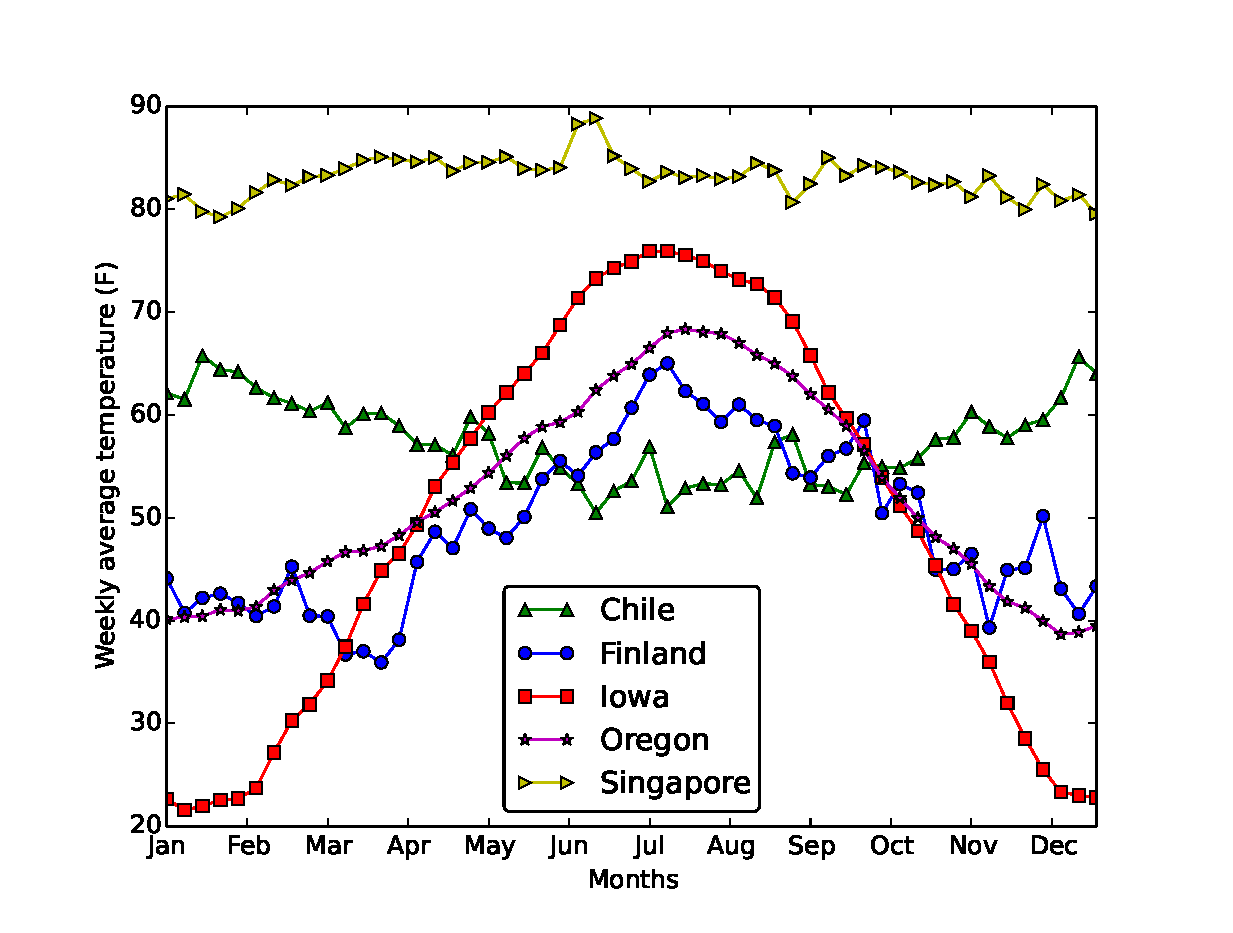
\includegraphics[scale=0.45]{temperature}
\caption{ Temperature variation for the year 2013}
 \label{fig:temp}
\end{figure}





\subsubsection{Temperature} \label{sec:temp}
Data centers located in cold regions have the advantage of using outside air to cool the data center. An air-side economizer brings outside air into a building and distributes it to the servers. Instead of being re-circulated and cooled, the exhaust air from the servers is simply directed outside. This can result in million dollars of saving annually. A difference in temperature across data centers leads to different cooling costs at these data centers. We wish to utilize this difference by scheduling jobs in low temperature data centers. In this case we make our assumption concrete by doing an empirical analysis of historical climate data. We extracted hourly temperature data from various data repositories of the National Climate Data Center \cite{climatedata} for all five locations covering the entire one-year period of 2013. Figure \ref{fig:temp} plots the weekly average temperature for five different locations in United States, Europe, South-America, and Asia. As expected we see high diversity in temperature at different locations. For example, Oregon and Finland seems to be equally favorable for cooling during most of the year except during the months of May {-} July. Chile and Singapore show almost no variation in temperature across the year. However, Chile is favorable for cooling conditions compared to Singapore.

\subsubsection{Electricity Pricing} \label{sec:elec}
Creation of power trading zones have resulted in wholesale power purchase under dynamic pricing schemes. Such markets are popular in USA \cite{elecusa}, Germany \cite{elecgermany} and other countries. Based on supply and demand bids there can be high fluctuations in prices \cite{benini2002day}. There are many ways to predict these prices \cite{contreras2003arima} \cite{garcia2005garch}. If we can predict the electricity prices for the job duration, then we will be able to schedule the job such that the running costs go down. Figure \ref{fig:elec} shows the variation in electricity prices across different data center regions in 2013. These price values have been consolidated from multiple sources on the Internet \cite{singelec} \cite{finelec} \cite{uselec}. For Chile, we were able to retrieve only monthly averages for 2013, but for all the other location we were successful in collecting hourly prices. From the figure \ref{fig:elec} it is clear that Singapore has the highest electricity pricing among all the regions under consideration. If we compare both figure \ref{fig:temp} and figure \ref{fig:elec} it is evident that Singapore is least suitable data center in terms of operational costs since the temperature and the energy prices are the highest. 

\begin{figure}[H]
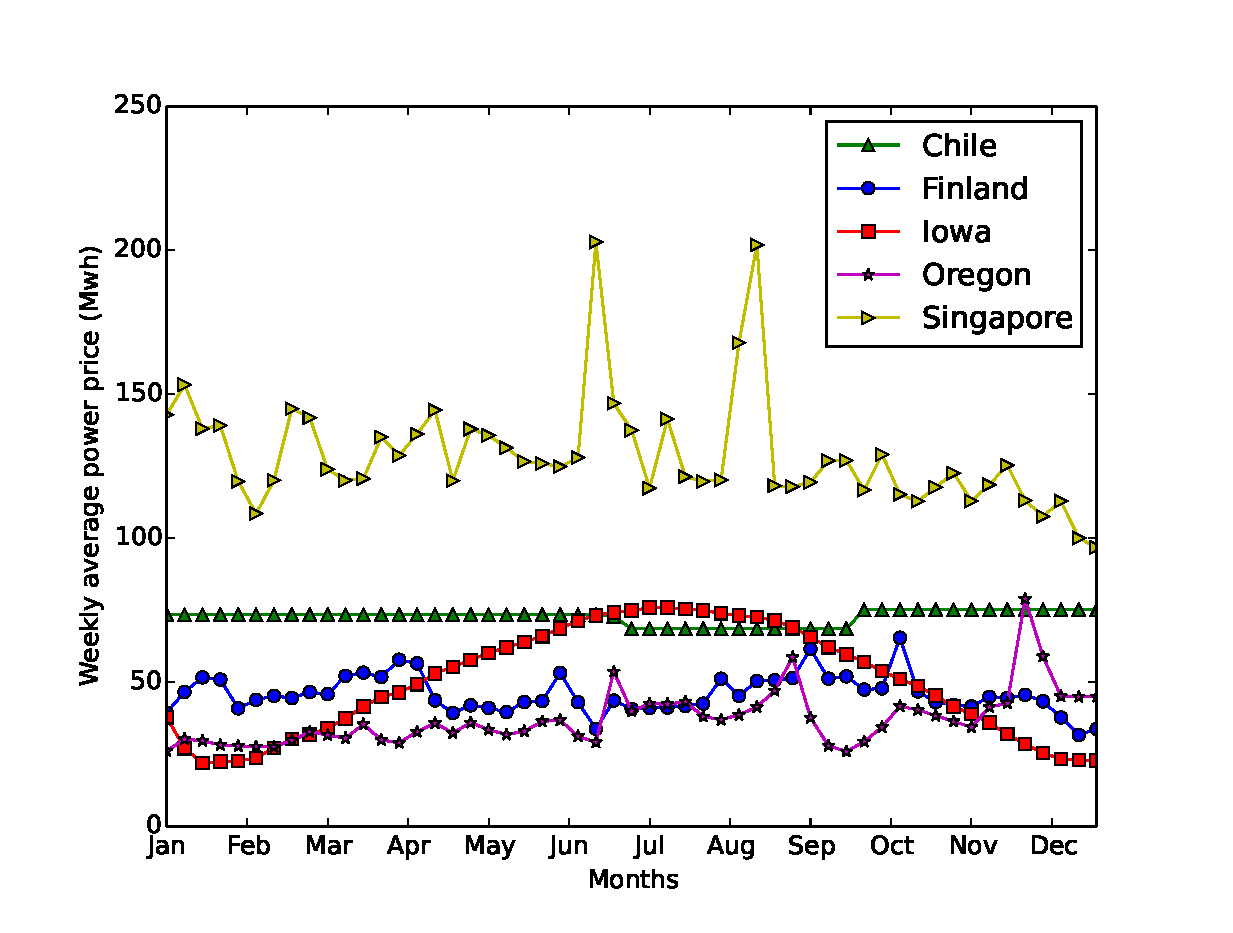
\includegraphics[scale=0.45]{elec}
\caption{ Electricity price variation for the year 2013}
 \label{fig:elec}
\end{figure}


\section{System Model}
\label{sec:sysmodel}
We model the total energy of the data center as a sum of energy consumed by the servers i.e IT equipments and the cooling subsystem. The subsection \ref{sec:servere} and \ref{sec:coole} provides more information about the model.

\begin{equation} \label{eq:etotal}
E_{total} = E_{server} + E_{cooling} 
\end{equation}

\subsection{Server Energy}
\label{sec:servere}
We model the power consumption of servers as the sum of power consumption of individual cores in the system. The power consumption on each core is the sum of the static power and the dynamic power needed to run computations. Eq \ref{eq:core} represents the power consumption of a core. Static power is consumed when the system is idle.

\begin{equation} \label{eq:core}
P_{core} = P_{static} + P_{dynamic} 
\end{equation}

The peak usage is when the cores are at the highest utilization. In cloud systems, it is very rare that the CPU utilization \textit{u} is more than 20\% \cite{birke2012data}. To account for this, we rewrite eq \ref{eq:core} as described in \cite{buyya2010energy}. 

\begin{equation} \label{eq:core_util}
P_{core}(u) = P_{static} + P_{dynamic_peak} * u 
\end{equation}

For our experiments we use the peak and idle power from \cite{kamil2008power}. The authors have characterized power usage of systems by running various HPC kernels. Since these kernels are CPU-intensive we can consider them to use the peak power. To emulate the CPU utilization of jobs, we generate random utilization based on the \textit{mean, standard deviation} and \textit{cov} provided in the work done on data center utilization by IBM \cite{birke2012data}.

The energy consumption of a job \textit{j} with core count \textit{c}, avgerage CPU utilization \textit{u} and running time \textit{t} is given in Eq \ref{eq:energy_job}

\begin{equation} \label{eq:power_job}
P_{j} = c*P_{core}(u)
\end{equation}

\begin{equation} \label{eq:energy_job}
E_{j} = P_{j}*t
\end{equation}


\subsection{Cooling Energy}
\label{sec:coole}
We model the energy consumption of the traditional CRAC as well as the air economizer in the sections below. 

\subsubsection{CRAC cooling units}
The power usage of CRAC units can be modeled using the equation  \ref{crac:eq} as given in \cite{christy2011energy}. The value of COP (coefficient of performance) can be calculated according to \cite{ahmad2010joint} using the equation \ref{eq:cop}. 

\begin{equation} \label{crac:eq}
P_{CRAC} = \frac{P_{dc}}{COP}
\end{equation}

\begin{equation} \label{eq:cop}
COP = 0.0068*(T_{sup}^2) + 0.0008*T_{sup} + 0.458
\end{equation}

In the above equations, ~$P_{dc}$ is the total power consumption of the data center and ~$T_{sup}$ is the temperature of the air supplied to the data center in degree Celsius.

\subsubsection{Air Economizer}

The power usage model for air economizer is given in \cite{christy2011energy}. The equation \ref{eq:aireco} represents the power consumption of the free air cooler. 


\begin{equation} \label{eq:aireco}
P_{air} = (PUE - 1) * P_{dc}
\end{equation}

The PUE(power usage effectiveness) is proportional to the outside temperature. We get the values of PUE from the product documentation of commercial vendors \cite{airecoproduct}. For our experiments, the value of PUE used is given in table \ref{tab:pue}.

\begin{table}[] 
 \centering
\begin{tabular}{|l|l|}
\hline
\bf{Temperature range (F)}      &       \bf{PUE} \\ \hline
less than 25  & 1.05    \\ \hline
25-35 & 1.07   \\ \hline
35-50 & 1.09    \\ \hline
50-60 & 1.10  \\ \hline
60-65 & 1.17  \\ \hline
\end{tabular}
\caption {PUE values for different temperature ranges} \label{tab:pue}
\end{table}

\subsection{Data center selection}
The data center is selected by calculating the power contributed by a job to the total server power consumption as well as cooling power. This is done by using Eq \ref{eq:power_job} in the power models for server and cooling. 
Equations \ref{eq:total_job_power}, \ref{eq:job_cost} and \ref{eq:job_min} show the mechanism of data center selection. 

\begin{equation} \label{eq:total_job_power}
P_{total}(j,dc) = P_{dynamic}(j,dc) + P_{cooling}(j,dc)
\end{equation}

\begin{equation} \label{eq:job_cost}
Cost(j,dc) = T_{j}*P_{total}(j,dc)*C_{mwh}(dc)
\end{equation}

\begin{equation} \label{eq:job_min}
dc_{j} = \min_{\forall dc \in DC} Cost(j,dc)
\end{equation}

The cost is the product of total power due to job ~$j$ in a specific data center ~$dc$, the running time of the job ~$T(j)$ and the electricity cost at the data center ~$C_{mwh}(dc)$. The data center corresponding to the minimum cost is selected for job scheduling as specified in Eq \ref{eq:job_min}.

%%%%%%%%%%%%%%%%%%%%%%%%%%%%%%%%%%%%%%%%%%%%%%%%%%%%%%%%%%%%%

\section{Evaluation}
\label{sec:eval}
\subsection{Simulator}
\label{sec:simdesign}
We evaluate our meta-scheduler by doing extensive simulations. For this purpose we developed a simulator \textit{GeoSim} which take in the workload trace and the data center profile as input and implements our model and routes jobs to the most cost effective data center. A brief overview of the design of \textit{GeoSim} is provided below. We have made the source code of \textit{GeoSim} and the workload traces public and is available at \cite{sourcecode} 

\

\subsubsection{Components}
\begin{list2} %Job Description%
\item \textbf{Datacenter:} This component will simulate a data center. This composed of 1) scheduler that implements a specific provisioning algorithm, 2) data center profile database, 3) a work trace reader and 4)proxy elements of other data center for inter-data center communication\
\item \textbf{DataCenter Proxy}: All interactions with the data center will be through a proxy. Each data center will hold the proxies to other data centers.\
\item \textbf{Scheduler:} This component will implement the model and schedule jobs onto data centers. We can experiment with different scheduling algorithms by plugging different Scheduler implementation\
\item \textbf{Datacenter Profile DB}: This components contains the temperature and electricity data. Scheduler will access this to make provisioning decisions.\
\end{list2}

\begin{figure}[] 
\centering
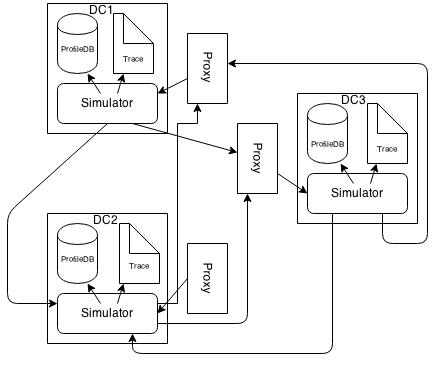
\includegraphics[scale=0.45]{comp_diag}
\caption{Simulation components and their interaction}
\label{fig:component}
\end{figure}

\subsubsection{Component Interaction}
Figure \ref{fig:component} gives the interaction model between the components. The data center object will start a thread which will run the scheduling algorithm, scheduling jobs from the trace file. Each data center has proxies to other data centers if it needs to communicate resource availability or job provisioning to other data centers. In our simulations we share resource utilization every 5 minutes, and each time step of the simulator is 5 seconds. These are provided as parameters to the simulator. Our simulations take around 4 hours to complete running on 6-core AMD Opteron(tm) server.

\begin{figure}[H]
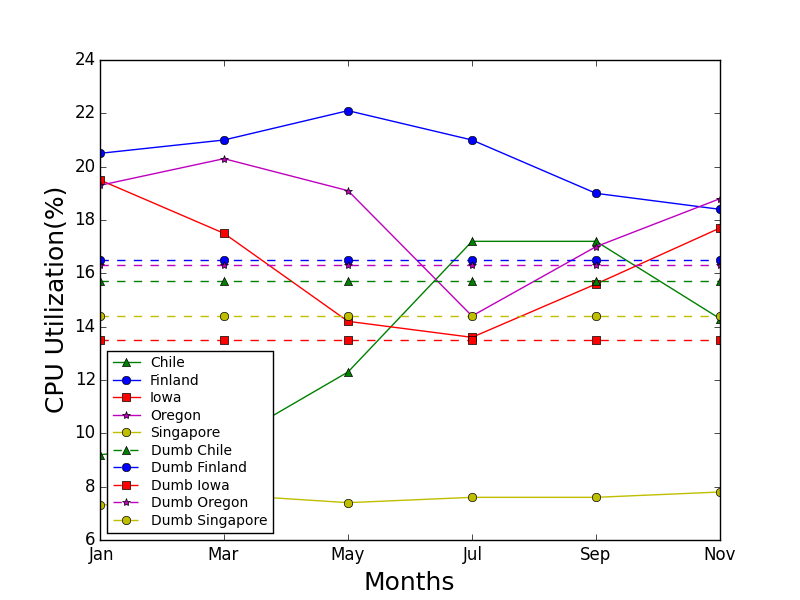
\includegraphics[scale=0.45]{cpu_util}
\caption{ Data center utilization}
 \label{fig:dcutil}
\end{figure}

\subsection{Results}
We run the simulations with GeoSched and also implement a naive scheduler called \textit{DumbSched} which schedules all the jobs to the local data centers. We will look at the cost saving as well as the energy savings with GeoSched. We will also look at the variation in utilization of each of the data centers across different months. We run the simulations for alternate months starting with January. We provide the date 15 and GMT time 12am as the start date and time for each simulation.

The results are summarized in table \ref{table:summary}. The total energy consumed by the data centers for 30 days (5 days in each of the 6 months) and the corresponding costs are shown. The energy  decrease by 8.2\% and the cost decrease by 11.7\%. When these results are extrapolated to 1 year the dollars  saved is around \$4.8 million. The experiments were run assuming a max core count in node to be 64. Since, Google traces normalize these values, it would be impossible to calculate energy with out an assumption.

\begin{table}[] 

 \centering
\begin{tabular}{|l|l|l|}
\hline
      &       \bf{Energy (MJ)} & \bf{Cost (\$)} \\ \hline
\bf{DumbSched} & 8044  & 560630   \\ \hline
\bf{GeoSched} & 7384 & 494560   \\ \hline
\bf{ Savings! } & 660 & 66070    \\ \hline
\end{tabular}
\caption {Result summary} \label{table:summary}
\end{table}


Figure \ref{fig:dcutil} shows the variation of data center utilization when the scheduling month changes. It is quiet evident that Singapore has the least utilization due to high operational costs. Similarly, the utilization at Iowa decreases towards may and increase towards the end of the year. This result is consistent with the temperature and electricity price data. Finland and Oregon has the highest utilization since these two have less operational cost as compared to the other three data centers. Chile, gets more jobs towards the middle of the year. This could be attributed to temperature increase in other data centers. 





Figure \ref{fig:dcenergy} shows the variation in energy consumption. It can be noted that some data centers consume more energy with GeoSched than DumbSched. This is because, in these data centers, more work can be done with less increase in energy consumption. Therefore, GeoSched will give a net decrease in energy consumption even if some data centers consume more energy than when scheduled using DumbSched.

\begin{figure}[H]
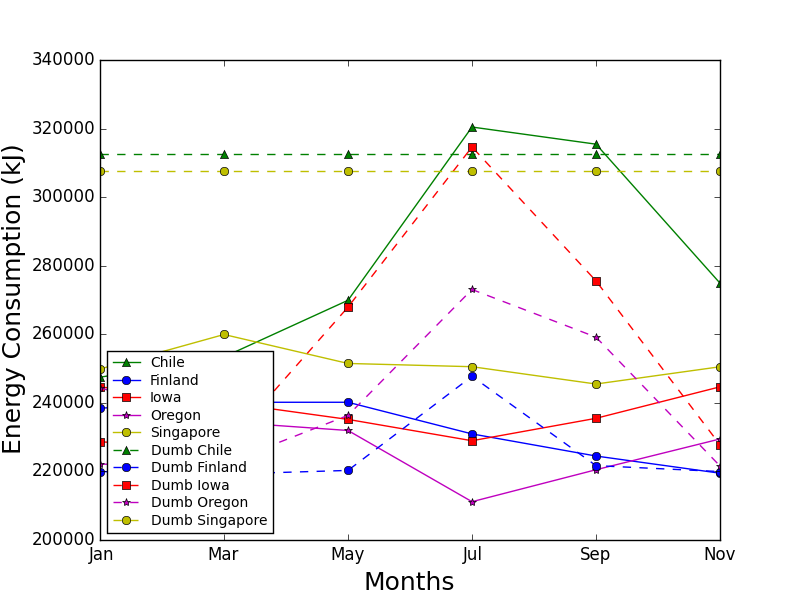
\includegraphics[scale=0.45]{energy}
\caption{ Variation in energy consumption}
 \label{fig:dcenergy}
\end{figure}

Figure \ref{fig:dccost} shows the cost of operation among different data centers. This plot can also be interpreted the same way as the energy consumption plot. There is a net gain in the cost of operating the data center when using GeoSched. More energy can be saved if the free nodes in the data center can be switched off. In our experiments, we always calculate the idle energy consumed by these machines.


\begin{figure}[]
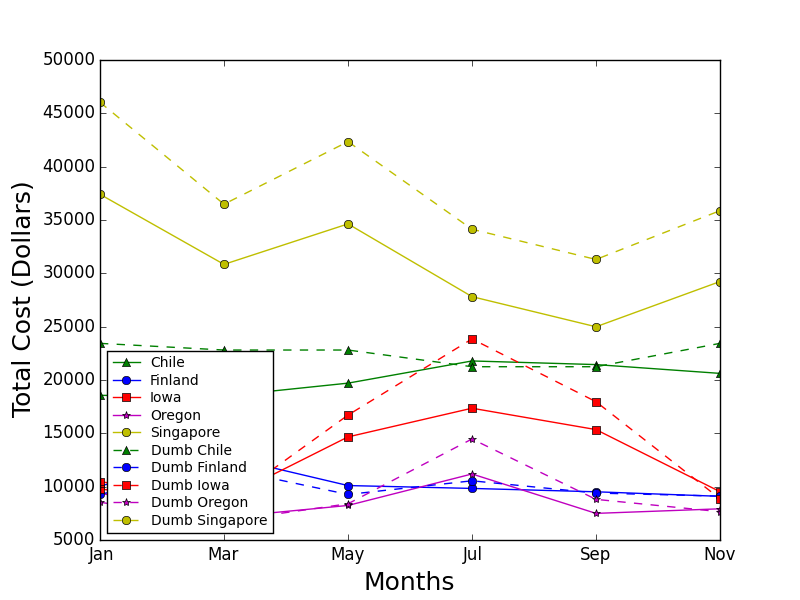
\includegraphics[scale=0.45]{dollars}
\caption{ Variation in operational cost}
 \label{fig:dccost}
\end{figure}

\section{CONCLUSION}
\label{sec:conclusion}
In this paper we build a meta-scheduler for geo-distributed data centers. We considered parameters like temperature and electricity prices to intelligently provision jobs to data centers. We evaluate our method using simulations and found our scheduler to reduce energy consumed by 8.2\% and the cost of operation 11.7\%. We wish to consider other factor influencing the energy consumption like availability of green energy and data transfer energy for our future work. We would also like to consider more descriptive SLAs to be included as part of our future work.

{\footnotesize \bibliographystyle{acm}
\bibliography{sample}}

% that's all folks
\end{document}


